\documentclass[a4paper, 12pt]{article}

%%% Работа с русским языком
\usepackage{cmap}					% поиск в PDF
\usepackage{mathtext} 				% русские буквы в формулах
\usepackage[T2A]{fontenc}			% кодировка		% кодировка исходного текста
\usepackage[english,russian]{babel}	% локализация и переносы

%%% Дополнительная работа с математикой
\usepackage{amsfonts,amssymb,amsthm,mathtools} % AMS
\usepackage{amsmath}
\usepackage{icomma} % "Умная" запятая: $0,2$ --- число, $0, 2$ --- перечисление

%% Номера формул
%\mathtoolsset{showonlyrefs=true} % Показывать номера только у тех формул, на которые есть \eqref{} в тексте.

%% Шрифты
\usepackage{euscript}	 % Шрифт Евклид
\usepackage{mathrsfs} % Красивый матшрифт

%% Перенос знаков в формулах (по Львовскому)
\newcommand*{\hm}[1]{#1\nobreak\discretionary{}
    {\hbox{$\mathsurround=0pt #1$}}{}}

%%% Работа с картинками
\usepackage{graphicx}  % Для вставки рисунков
\graphicspath{{images/}{images2/}}  % папки с картинками
\setlength\fboxsep{3pt} % Отступ рамки \fbox{} от рисунка
\setlength\fboxrule{1pt} % Толщина линий рамки \fbox{}
\usepackage{wrapfig} % Обтекание рисунков и таблиц текстом

%%% Работа с таблицами
\usepackage{array,tabularx,tabulary,booktabs} % Дополнительная работа с таблицами
\usepackage{longtable}  % Длинные таблицы
\usepackage{multirow} % Слияние строк в таблице


\usepackage[utf8]{inputenc}
\usepackage[russian]{babel}
\usepackage{amsmath,amsfonts,amssymb,amsthm,mathtools} %AMS

\usepackage{hyperref}  % Гиперссылки
\usepackage[usernames,dvipsnames,svgnames,table,rgb]{xcolor}
\usepackage{enumitem} %Для нумерации списков
\usepackage{multicol} % Несколько колонок

\hypersetup{
    unicode=true,
    pdftitle={cheat_sheet}, % Заголовок
    pdfauthor={Кузьмин Никита, ММП 317},
    pdfcreator={Кузьмин Никита, ММП 317},
    colorlinks=false, % false - ссылки в рамках; true - цветные ссылки
    linkcolor=red,   % внутренние ссылки
    citecolor=green, % на библиографию
    filecolor=magenta, % на файлы
    urlcolor=blue % на URL
}

\usepackage{fancyhdr} % Колонтитулы
%\pagestyle{fancy}

\begin{document}
    
    \thispagestyle{empty}
    \begin{center}
        \textit{Московский Государственный Университет имени М. В. Ломоносова\\
            Факультет выислительной математики и кибернетики}
        \vspace{0.5ex}
        \vspace{30ex}
        
        Отчет по заданию №1 "\textbf{Метрические алгоритмы классификации}". Алгоритм k ближайших соседей
        
    \end{center}
    \vspace{13ex}
    \begin{flushright}
        \noindent % Убирает красную строку
        \vfill
        \textit{Кузьмин Н. В.}
        \\
        \textit{студент кафедры ММП \\ 317 группа}
        
    \end{flushright}
    \begin{center}
        Октябрь,
        
        2019
    \end{center}
    \newpage
    \begin{center}
        \textbf{Содержание}
    \end{center}
    %\begin{enumerate}
    %    \item Введение
    %    \item Эксперименты
    %    \begin{enumerate}[label*=\arabic*.]
    %        \item Скорость поиска ближайших %соседей
    %        \item Зависимость точности %модели от количества соседей и %метрики
    %        \item Сравнение точности %взвешенного метода и метода без %весов
    %        \item Анализ модели с лучшим %качеством
    %        \item Применение трансформаций %к тренировочной выборке
    %         \begin{enumerate}[label*=\arab%ic*.]
    %            \item Повороты
    %            \item Смещения
    %            \item Фильтр Гаусса
    %         \end{enumerate}
    %         \item Применение трансформаций %к тестовой выборке
    %         \begin{enumerate}[label*=\arab%ic*.]
    %            \item Повороты
    %            \item Смещения
    %            \item Фильтр Гаусса
    %         \end{enumerate}
    %    \end{enumerate}
    %    \item Бонусная часть
    %    \item Выводы
    %\end{enumerate}
    \tableofcontents
    
    \newpage
    \section{Введение}
    В этом документе представлен отчет о проделанных экспериментах по практическому заданию №1, анализ результатов.
    
    \section{Эксперименты}
    В этом блоке приведены все обязательные эксперименты, которые изложены в формулировке задания.
    \subsection{Скорость поиска ближайших соседей}
    \subsubsection{Дизайн эксперимента:}
    Были протестированы 4 алгоритма поиска 5 ближайших соседей с разными размерами признакового пространства:
    
    Алгоритмы: \hfill Размеры признакового пространства: % добавить еще маркированный список
    \begin{itemize}
        \begin{multicols}{2}
            \item \text{<<my\_own>>}
            \item \text{<<brute>>}
            \item \text{<<kd\_tree>>}
            \item \text{<<ball\_tree>>}
            \item 10
            \item 20
            \item 100
        \end{multicols}
    \end{itemize}
    \subsubsection{Ожидания}
    Ожидается, что <<kd\_tree>>, <<ball\_tree>> будут очень хорошо работать для маленького количества признаков, но с увеличением размерности признакового пространства произойдет резкое увеличение скорости работы.
    \subsubsection{Результаты}
    Подробные результаты экспериментов приведены в таблице \ref{exp1:table}:
    \\
        \begin{table}[h!]
            \begin{center}
                \caption{Результаты эксперимента №1} \label{exp1:table}
                \begin{tabular}{|c|c|r|} 
                    \hline 
                    размерность & алгоритм & время работы \\ 
                    \hline
                    10 & my\_own & 68.07 \\ 
                    \cline{2-3} 
                    & brute & 7.84 \\ 
                    \cline{2-3} 
                    & \textbf{kd\_tree} & \textbf{0.44} \\ 
                    \cline{2-3} 
                    & ball\_tree & 1.72 \\ 
                    \cline{2-3} 
                    \hline 
                    20 & my\_own & 76.82 \\ 
                    \cline{2-3}  
                    & brute & 7.95 \\ 
                    \cline{2-3}  
                    & \textbf{kd\_tree} & \textbf{1.40} \\ 
                    \cline{2-3} 
                    & ball\_tree & 6.63 \\ 
                    \hline 
                    100 & my\_own & 78.31 \\ 
                    \cline{2-3}  
                    & \textbf{brute} & \textbf{8.28} \\ 
                    \cline{2-3} 
                    & kd\_tree & 82.76 \\ 
                    \cline{2-3}
                    & ball\_tree & 97.67 \\
                    \hline
                \end{tabular} 
            \end{center}
        \end{table}
    %%вставить табличку
    \subsubsection{Выводы}
    Самым стабильным алгоритмом оказался <<brute>>, который практически не деградирует с ростом размерности. Как и ожидалось, алгоритмы, реализованные на деревьях, сильно замедлились на признаковом пространстве размерности 100.
    
    \subsection{Зависимость точности модели от количества соседей и метрики}
    \subsubsection{Дизайн эксперимента}
    В этом эксперименте была рассмотрена зависимость точности и времени работы модели k ближайших от следующих параметров на 3 валидационных фолдах:
    \begin{itemize}
        \item k от 1 до 10 (только влияние на точность).
        \item Евклидова или косинусная метрики.
    \end{itemize}
    
    
    \subsubsection{Результаты}
        Зависимость средней точности от числа соседей для различных метрик приведена на графике \ref{exp2:graph}
        
        Измерения скорости для евлидовой и косинусной метрик приведены в таблице \ref{exp2:speed}
    \begin{figure}
        \caption{}\label{exp2:graph}
        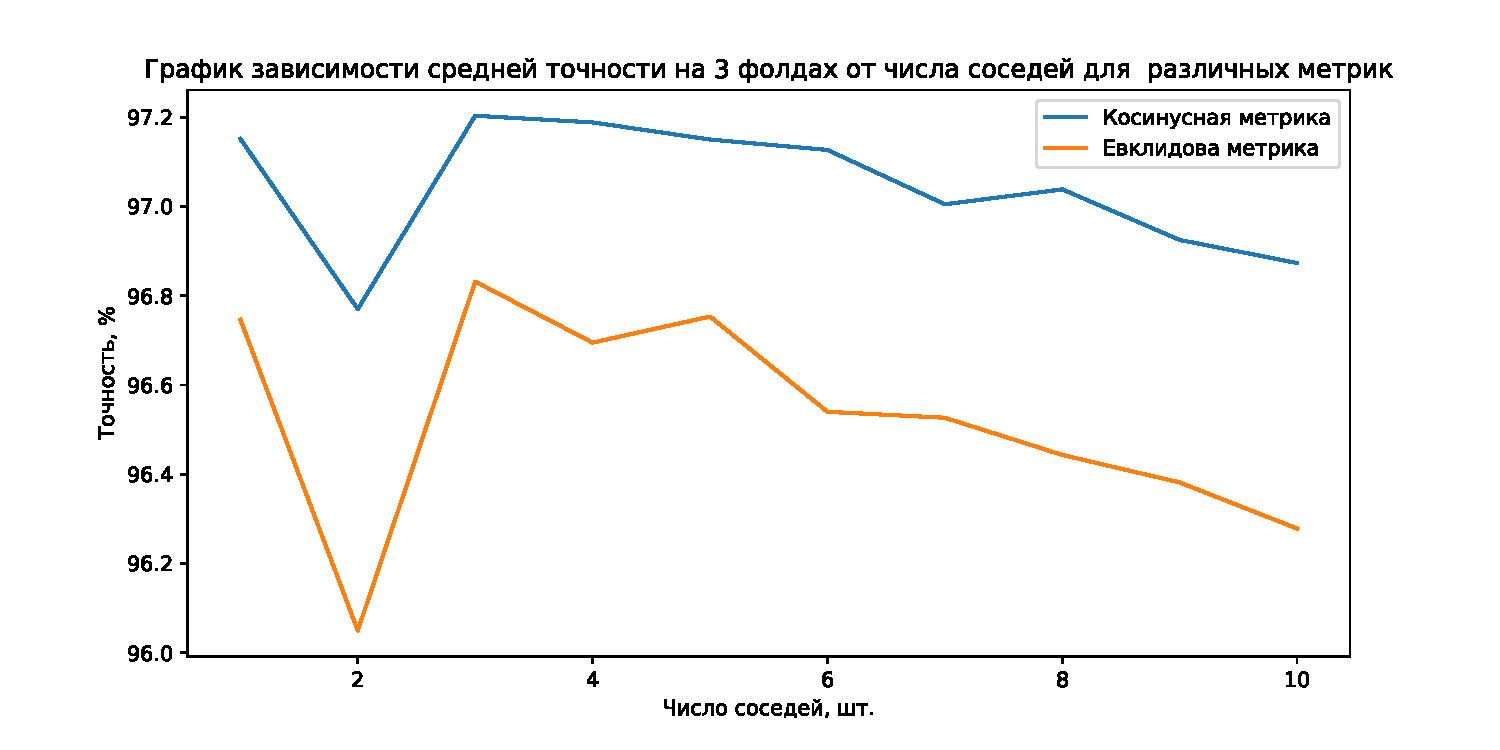
\includegraphics[width=\textwidth]{../experiment2_graph.pdf}
    \end{figure} 
    
    \begin{table}[h]
        \begin{center} 
            \caption{Скорость работы метрик (измеренная при кросс-валидации на 3 фолдах)} \label{exp2:speed}
            \begin{tabular}{|c|c|}
                \hline 
                метрика & время \\ 
                \hline 
                евклидова & 103.42 \\ 
                \hline 
                косинусная & 101.69 \\ 
                \hline 
            \end{tabular}
        \end{center}
    \end{table}
    
    \subsubsection{Выводы}
    Из графика \ref{exp2:graph} видно, что:
        \begin{enumerate}
            \item Наилучшая точность алгоритма достигается при $k = 3$ для обеих метрик.
            \item С увеличением количества соседей (при $k \ge 5$) точность начинает убывать.
        \end{enumerate} 
    Из таблицы \ref{exp2:speed} видно, что скорость работы алгоритмов практически не зависит от выбора данных метрик
    \subsection{Сравнение точности взвешенного метода и метода без весов}
    \subsubsection{Дизайн эксперимента}
    \subsubsection{Результаты}
    Результаты эксперимента №3 приведены на графике \ref{exp3:graph}
    \begin{figure}
        \caption{}\label{exp3:graph}
        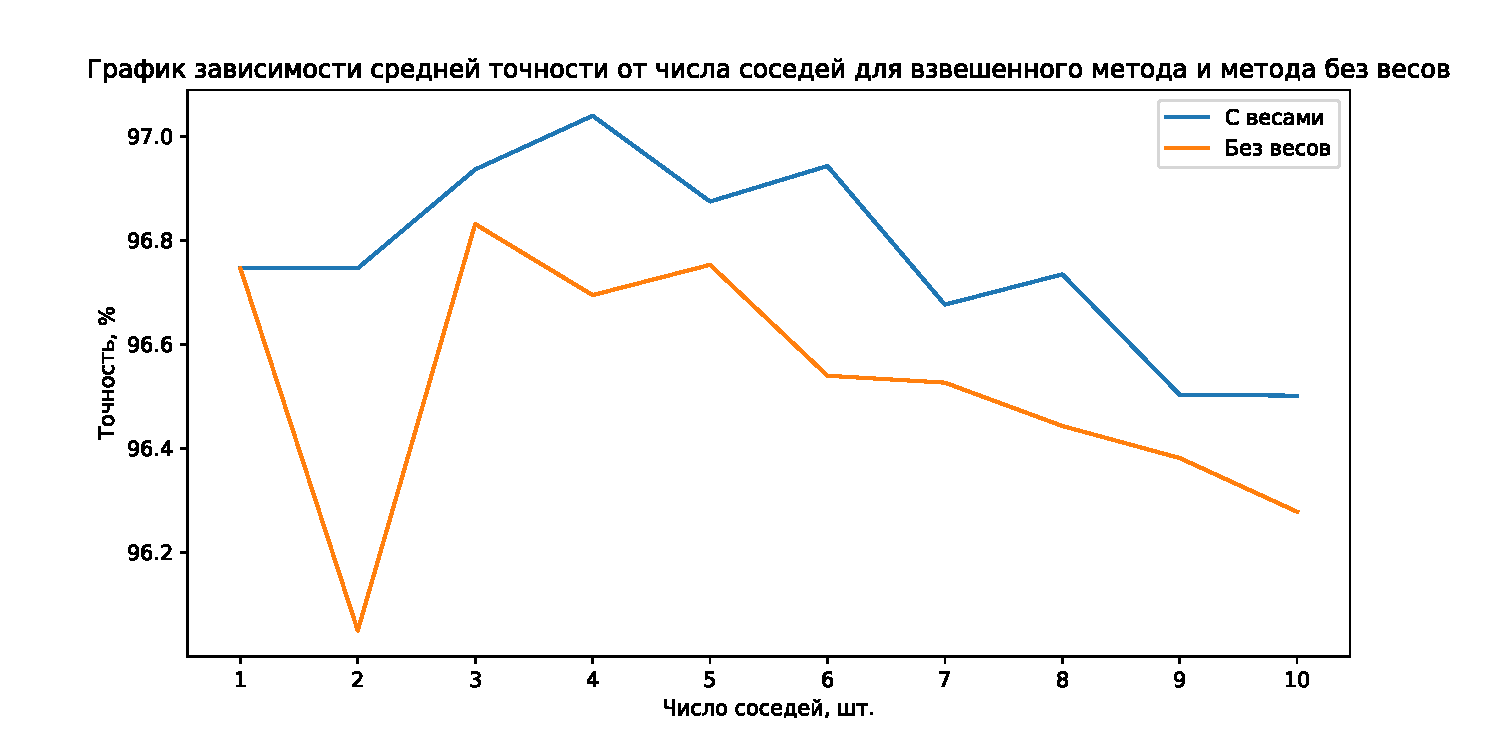
\includegraphics[width=\textwidth]{../experiment3_graph.pdf}
    \end{figure} 
    \subsubsection{Выводы}
    По графику \ref{exp3:graph} можно заметить, что взвешенный метод лучше по точности во всех случаях, кроме $k = 1$, что является логичным, так как в этой ситуации веса бесполезны.
    \subsection{Анализ модели с лучшим качеством}
    \subsubsection{Дизайн эксперимента}
    Применим лучший алгоритм к исходной обучающей и тестовой выборке и проанализируем матрицу ошибок (confusion matrix).
    \subsubsection{Результаты}
    Матрица ошибок представлена на рисунке №, Визуализированные объекты - на рисунке №
    \subsubsection{Выводы}
    Можно увидеть, что самые частые ошибки происходят на парах цифр, представленных ниже:
    \begin{itemize}
        \begin{multicols}{2}
            \item 4 и 9
            \item 3 и 5
            \item 1 и 7
            \item 3 и 8
        \end{multicols}
    \end{itemize}
    Эти пары похожи по написанию, поэтому алгоритму тяжелее отличить их друг от друга. 
    
    Рассмотрим теперь объекты, на которых произошли ошибки. У них можно заметить характерные особенности:
    \begin{enumerate}
        \item Засечки
        \item Крючки
        \item Разные деформации
    \end{enumerate}
    В большинстве случаев видно, что написаннные цифры немного деформированы и похожи на другие в некоторых чертах. Эти особенности затрудняют классификацию для алгоритма.
    \\
    
    
\end{document}

